\markboth{Age model}{Age model}
\section{Age model}
The age model is implemented using the Observer design pattern via Matlab's "Events and Listeners\footnote{in \matlab, an observer is often referred to as a "listener". However, "observer" is the more common term in OOP design pattern terminology and will be used throughout this documentation.}"~\cite{_overview_????}. This way, various age models (predefined or custom) can be dynamically added to a battery model at run time or even left out completely. Ageing can be simulated on the battery pack level (by treating all cells as one entity) or on the cell level (by observing each cell separately). The event oriented age model provided in this package is based solely on cycle counting, for which a mathematical approach developed by~\cite{dambrowski_mathematical_2012} is implemented. Descriptions of the counting algorithm and the classes used to implement the age model are provided in the following sections.
\subsection{Overview}
Cycle counting algorithms are designed to count cycles from a set of measured data. A challenge for a running simulation or a battery management system (BMS) that relies on cycle counting is to decide when to count the cycles of an accumulated data set. Counting could be done at fixed time intervals or it could be triggered by a certain event. The latter is the approach implemented by the \mcode{cycleCounter} interface, which acts both as an observer of a battery cell or pack as well as a subject for the \mcode{eoAgeModel} class.\\
The observation of charge cycles is handled by the abstract \mcode{cycleCounter} interface, in which all methods except for the \mcode{count()} method are predefined. An object that implements the interface is regularly updated with the observed battery's $SoC$, which is stored within the object's memory. The cycle counting occurs every time the $SoC$ reaches an upper threshold, i.e. the observed battery's maximum $SoC$. After counting, the \mcode{NewCycle} event is triggered, causing all of the object's observers (i.e. an \mcode{eoAgeModel} object) to be notified that new data is available for simulation. The age model then uses the data to determine the battery's new state of health $SoH$ and passes it on to the battery. \\
An Observer Pattern class diagram of the age model is depicted in Figure~\ref{fig:observer_schema}. The observation is handled by the respective abstract interfaces, while the actual simulation is handled by the implementations. This makes the model highly flexible. For example, a lightweight implementation could be to observe a \mcode{batteryPack} using a single \mcode{cycleCounter} and a single \mcode{batteryAgeModel}. Another option could be to use multiple \mcode{cycleCounter} and \mcode{ageModel} objects in order to simulate the ageing of each \mcode{batteryCell} within a pack individually. The cycle counting can be implemented by various algorithms (two are provided in this package). And advanced users could even replace the default age model implementation (\mcode{eoAgeModel}) with a custom class that takes other factors into account, e.g. calendar ageing or thermal influences. In large simulations, it may be of interest to neglect the battery ageing in order to save simulation time. This can either be done by simply not linking up the components at runtime or by including a \mcode{dummyCycleCounter} and a \mcode{dummyAgeModel}. These classes implement the \mcode{cycleCounter} and \mcode{batteryAgeModel} interfaces, respectively. However, calling their methods does nothing. The former option is faster, due to reduced method overhead, but the latter may be more robust in some cases.
\begin{figure}[t!]
	\captionsetup{type=figure}
	\centering
	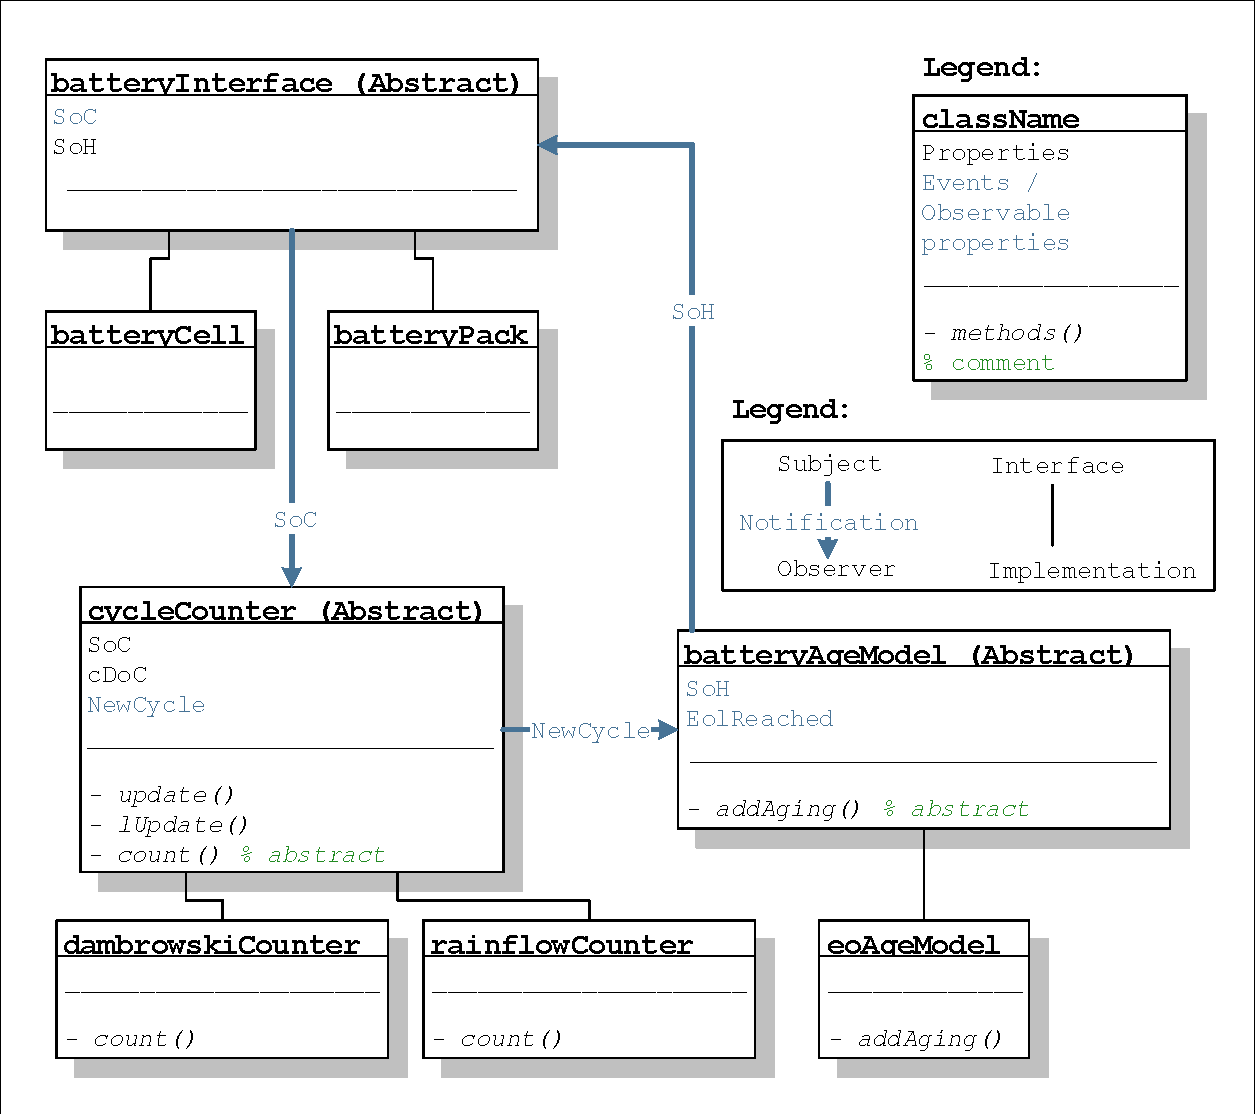
\includegraphics[width=\textwidth]{observer_schema.pdf}
	\caption[Overview of the Observer implementation of the age model with communication flows and inheritance links]{Overview of the Observer implementation of the age model with communication flows and inheritance links.}
	\label{fig:observer_schema}
\end{figure}

\subsection{Cycle counting}
In this pack, two classes have been created to implement the \mcode{cycleCounter}'s \mcode{count()} method.
A \mcode{cycleCounter} subclass can be constructed in one of the following ways:
\begin{lstlisting}
c = cycleCounter; % sets the initial SoC to 0.2 and the max. SoC to 1
c = cycleCounter(init_soc); % sets the initial SoC
c = cycleCounter(init_soc, soc_max); % sets the initial SoC and the
									 % max. SoC
\end{lstlisting}
where \mcode{cycleCounter} must be replaced with the name of the respective class that is being constructed (e.g. \mcode{dambrowskiCounter} or \mcode{rainflowCounter}). To register the object as an observer of a battery object \mcode{bat}\footnote{\mcode{bat} can be an object of any class that implements the \mcode{batteryInterface}.}\todo{ref section}, the \mcode{initAgeModel()} method can be used.
\begin{lstlisting}
% Extract intitial SoC and max. SoC from battery
init_soc = bat.SoC;
soc_max = bat.socMax;
% Replace "cycleCounter" with the respective subclass
c = cycleCounter(init_soc, soc_max);
% Intitialize event oriented age model with cycle counter c
bat.initAgeModel('ageModel', 'EO', 'cycleCounter', c)
\end{lstlisting}
Note that the \mcode{'ageModel'} option must be specified, otherwise \mcode{bat} will internally replace \mcode{c} with a \mcode{dummyCycleCounter} object to prevent runtime errors. If this happens, a warning message is printed to the command window.

\subsubsection{The \mcode{rainflowCounter} class}
The state of the art algorithm for cycle counting, "rainflow", was originally developed for mechanical stress modelling~\cite{matsuishi_fatigue_1968} and has recently become popular in the field of battery charge cycle counting~\cite{dufo-lopez_multi-objective_2008}. The \mcode{rainflowCounter} class was added to this package for the purpose of demonstrating the flexibility of the age model implementation. It acts as an adapter for the popular FileExchange contribution, "Rainflow Counting Algorithm" by Adam Nieslony~\cite{_rainflow_????}. In order for the class to work, the MEX functions must be downloaded from \cite{_rainflow_????} and placed within Matlab's search path. They are not included in this package and attempting to construct a \mcode{rainflowCounter} object will fail if they are not found. To register a \mcode{rainflowCounter} with a battery \mcode{bat}, the above syntax must be used, whereby \mcode{cycleCounter(init_soc, soc_max)} is replaced by \mcode{rainflowCounter(init_soc, soc_max)}.

\subsubsection{The \mcode{dambrowskiCounter} class}
In 2012, J.~Dambrowski, S.~Pichlmaier and A.~Jossen developed a mathematical definition of a battery's charge cycles along with an algorithm for counting them~\cite{dambrowski_mathematical_2012}. Since the counting algorithm was not named, the \mcode{dambrowskiCounter} class that implements it in this package was named after one of the authors. In their approach, so-called pre-cycles are counted and compared with each other. This is visualized in Figure~\ref{fig:pre_cycles}. The twice depicted $SoC$ curve (grey) has two local maxima $SoC\subs{max,l}{i}$, since the last value is counted as a local maximum. Starting from an $SoC\subs{max,l}{i}$, a pre-cycle of "prior equality" is defined as the $SoC$ within an interval between the respective  $SoC\subi{max,l}$ and the last point at which the $SoC$ was equal to  $SoC\subi{max,l}$. Two such pre-cycles are depicted in Figure~\ref{fig:pre_cycles} (left) and coloured in red and blue, respectively. A pre-cycle of "subsequent equality" (Figure~\ref{fig:pre_cycles}, right, coloured in blue) is defined as the $SoC$ within an interval between the respective $SoC\subi{max,l}$ and the subsequent point at which the $SoC$ is equal to $SoC\subi{max,l}$. Finally, a pre-cycle is counted as a cycle if there is no larger pre-cycle that encompasses the same interval and shares the same local minimum. This is not the case for the small cycle (coloured red) in Figure~\ref{fig:pre_cycles} (left); so the depicted curve contains two cycles. \\ \\
\begin{centering}
	\begin{figure}[t!]
		\subfloat{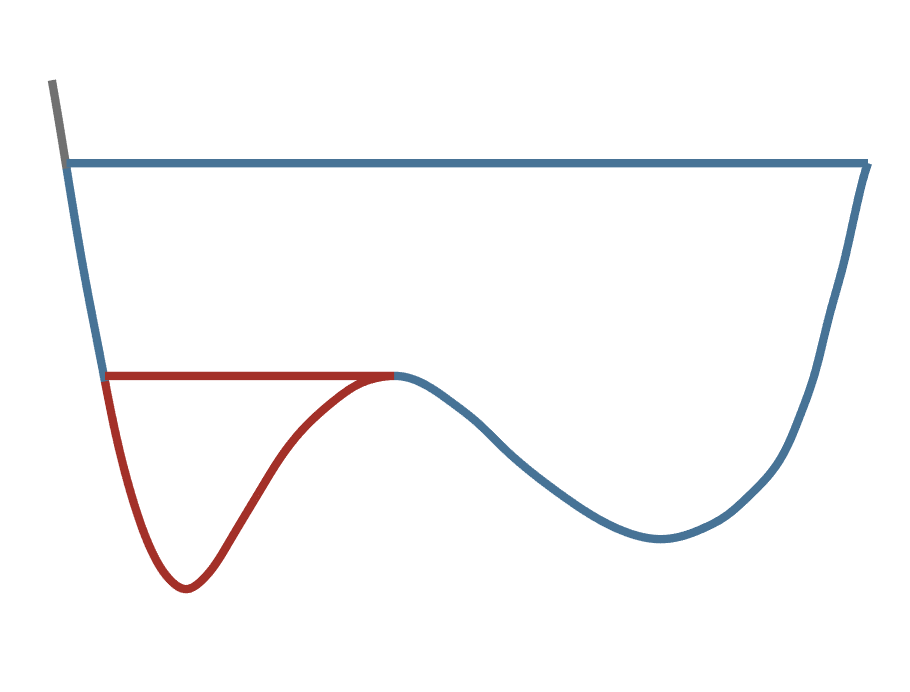
\includegraphics[width=0.5\textwidth]{DAM01}}
		\subfloat{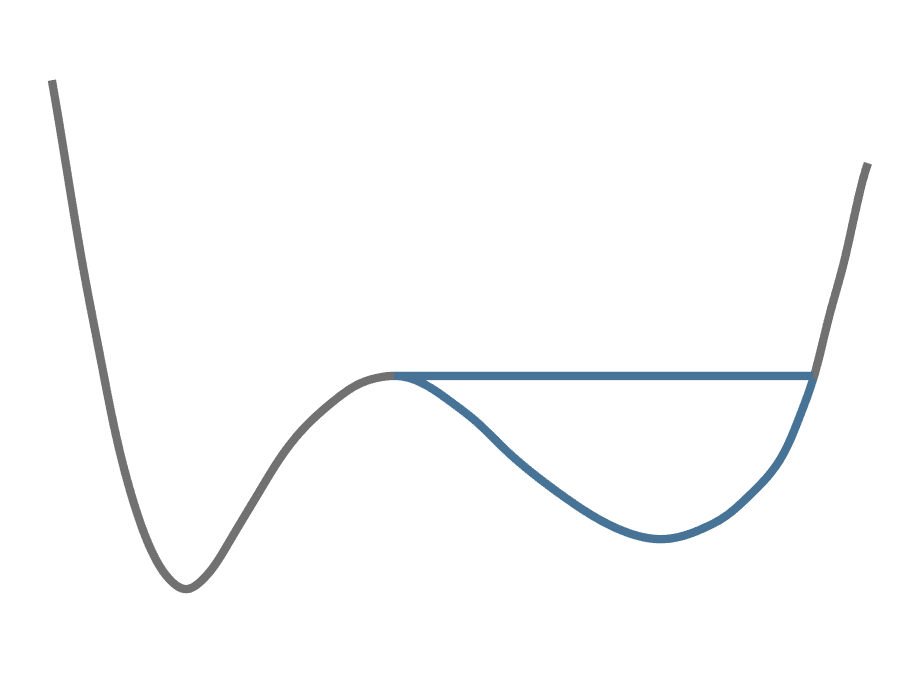
\includegraphics[width=0.5\textwidth]{DAM02}}
		\captionsetup{type = figure}
		\caption[Qualitative visualization of pre-cycle counting: Two pre-cycles of prior equality and a pre-cycle of subsequent equality]{Qualitative visualization of pre-cycle counting according to~\cite{dambrowski_mathematical_2012}: Two pre-cycles of prior equality (left) and a pre-cycle of subsequent equality (right).}
		\label{fig:pre_cycles} 
	\end{figure}
\end{centering}
In this package, \mcode{dambrowskiCounter} is the default cycle counter if an age model is specified. Thus, it does not have to be passed as an argument in a battery's \mcode{initAgeMode()} method.
\begin{lstlisting}
bat.initAgeModel('ageModel', 'EO')
% Automatically initializes a dabrowskiCounter object with init_soc
% and soc_max set according to the battery's properties and links.
\end{lstlisting}

\subsubsection{Comparison of the cycle counters}
Each \mcode{cycleCounter} object's \mcode{count()} method converts the saved $SoC$ profile into a cycle-Depth-of-Cycle $cDoC$ curve - a vector containing the depths of discharge $DoD$ of all the counted cycles. The simulation results of two batteries using a \mcode{dambrowskiCounter} and a \mcode{rainflowCounter}, respectively, are compared in Figure~\ref{fig:cdoc_hists}. The cycles' $DoD$s are each sorted into 50 BINs and compared in a histogram. Overall, the histograms appear very similar, thus proving that both classes produce good results. However, more cycles are counted using the \mcode{dambrowskiCounter} class, possibly causing the simulated battery to age slightly faster. While both classes use different methods for determining the extrema\footnote{\mcode{dambrowskiCounter} uses \mcode{cycleCounter}'s \mcode{iMaxima()} method and \mcode{rainflowCounter} uses the \mcode{sig2ext()} function~\cite{_rainflow_????}.}, the amount local maxima found is the same. Thus, the determination of extrema can be ruled out as a cause and the root of the discrepancy must lie within the different counting approaches.
\begin{figure}[t!]
	\captionsetup{type=figure}
	\centering
	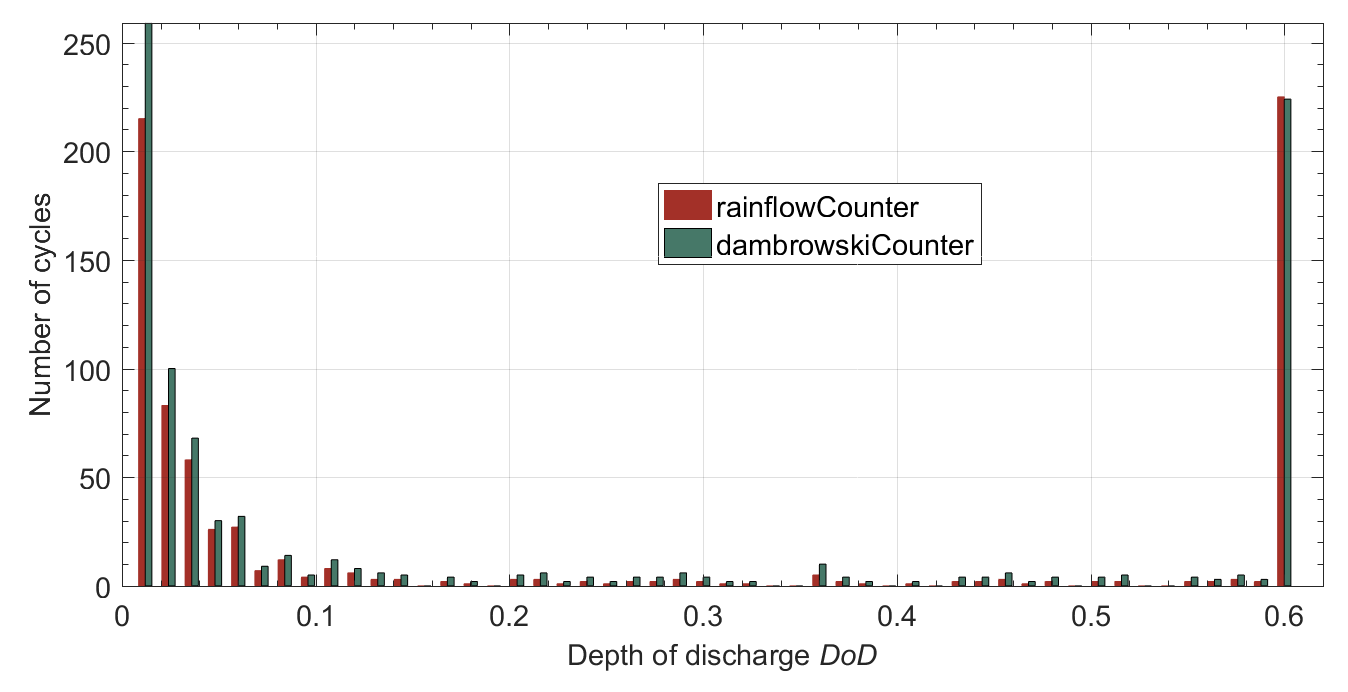
\includegraphics[width=\textwidth]{cdoc_hists}
	\caption[Comparison of the counted cycles and their $DoD$ between two simulations using the \mcode{rainflowCounter} and the \mcode{dambrowskiCounter} using the same $SoC$ profile]{Comparison of the counted cycles and their $DoD$ between two simulations using the \mcode{rainflowCounter} and the \mcode{dambrowskiCounter} using the same $SoC$ profile.}
	\label{fig:cdoc_hists}
\end{figure}

\subsection{Event oriented ageing model}
The event oriented ageing model - a very simple and lightweight model - is implemented by the \mcode{eoAgeModel} class, which subclasses the abstract \mcode{batteryAgeModel} interface.


\subsection{Creating a user-defined age model}
\begin{lstlisting}
classdef myCalendarAgeModel < lfpBattery.eoAgeModel
%MYCUSTOMAGEMODEL: An example for a user-defined age model.
%Combines the event oriented age model with a linear calendar age model.

	properties
		L_cal; % calendar life in s
	end
	
	methods
		function obj = myCalendarAgeModel(l, varargin)
			% l = calendar life in years
			% varargin = input args of eoAgeModel constructor
			%% call superclass constructor
			obj = obj@lfpBattery.eoAgeModel(varargin{:});
			obj.L_cal = l * 31557600; % set L_cal in seconds
		end
		function addCalAge(obj, dt)
			% Adds to the battery's age using the simulation time
			% step size.
			% dt = simulation time step size in s
			% obj.Ac = 1 - obj.SoH
			obj.Ac = obj.Ac + dt / obj.L_cal; % increment age
	 	end
	 end
end
\end{lstlisting}
